\addcontentsline{toc}{section}{Introduction}
\section*{Introduction}

Le concept de la formation à distance ne date pas d’hier. 
Dans ce chapitre, nous ferons une revue des origines de cette méthode d’enseignement. 
S’en suivra une analyse des techniques modernes de communication en temps réel et des solutions existantes qui permettent  de dispenser des cours à distance.

\section{Formation à distance}

L'encyclopédie Wikipedia définit la formation à distance comme une 
forme d’enseignement ou l’enseignant et l'étudiant sont séparés 
dans le temps et/ou par l’espace \cite{distance_education}.

\subsection{Origines}

Les premiers essais de formation à distance remontent à bien avant l'ère moderne. 
En effet, déjà en 1728, Caleb Phillips, un professeur, 
recherchaient des étudiants désirant acquérir des compétences en sténographie, 
auxquels il dispensait les cours par courrier.

Au sens moderne, le premier cours d’enseignement à distance, est attribué à Isaac Pitman, toujours en rapport avec la sténographie. 
Un nouvel élément qui apparaît dans le cas actuel, c’est la rétroaction des étudiants, 
qui devaient envoyer leurs transcriptions par la poste, pour correction. 
Ce mode de fonctionnement fut rendu possible par l’uniformisation des tarifs postaux en Angleterre. 
Plusieurs institutions telles que Oxford et l'université de Londre ont également expérimenté l’enseignement à distance.

Aujourd’hui, l’expansion d’Internet et du World Wide Web, permettent la mise en œuvre des moyens toujours plus sophistiqués, pour dispenser les cours à distance.


\subsection{Internet et formations en ligne}

L'avènement des nouvelles technologies de l’information et de la communication 
a donné lieu à la mise en place des formations en ligne, 
une forme évoluée de formation à distance \cite{online_learning}. 
En 2020, par exemple, sous l’impulsion de la pandémie alors en cours, 
plusieurs universités dont celle d’Abomey-Calavi, 
effectuent la transition partielle ou totale vers les classes virtuelles \cite{etudiant_dot_bj}.

On distingue deux environnements d’apprentissage. 
D’une part, les environnements asynchrones, qui offrent une totale liberté à l'apprenant quant à la gestion de son temps. 
L’enseignant et lui sont séparés littéralement par le temps et la distance. Ainsi, il peut consulter les ressources au moment qui lui convient le mieux. 
Cela permet une assimilation plus facile, étant donné que chaque apprenant peut s’adapter en fonction de ses besoins spécifiques. 
Toutefois, il est possible que l’apprenant se retrouve isolé et ne fasse finalement aucun progrès, faute de support.

D’autre part, un environnement synchrone essaie d'émuler une classe présentiel, 
à la seule différence que les participants sont physiquement distants. 
Avec des outils de messagerie instantanée et/ou de visioconférence, 
les apprenants peuvent interagir avec leurs pairs ainsi que le ou les enseignants.

En termes de classification des diverses formes de cours en ligne, Andreas Kaplan, 
auteur du livre \textit{Contemporary Issues in Social Media Marketing} \cite{andreas_kaplan_classfication}, propose une approche simplifiée basée sur les facteurs 
comme le temps, la distance et le nombre d’apprenants. 
Le tableau \ref{table:andreas_k_dot} en fait un récapitulatif.

\begin{table}[h!]
  \centering
\begin{tabular}{|l|l|l|}
  \hline
  Type de cours &  Nombre d’apprenants &  Type d’environnement \\
  \hline
  \acrfull{mooc} & illimité(en théorie) & asynchrone \\
  \hline
  \acrfull{smoc} & illimité(en théorie) & synchrone \\
  \hline
  \acrfull{spoc} & limité & asynchrone \\
  \hline
  \acrfull{ssoc} & limité & synchrone \\
  \hline
\end{tabular}
\caption{Classfication des types de formations en ligne}
\label{table:andreas_k_dot}
\end{table}

Notons que notre étude s'intéresse notamment aux environnements d’apprentissage synchrones, 
avec le support d’un grand nombre d’apprenants.

\section{Communication en temps réel}
Les outils de communications en temps réel désignent une catégorie de logiciels qui garantissent le traitement et la transmission instantanée, 
ou avec un délai fortement négligeable,  de l’information. 
Parmi les protocoles permettant ce type de communication, le plus en vogue reste \acrfull{webrtc}.


\acrshort{webrtc} est un protocole open source de transmission \acrfull{p2p}, qui assure la transmission de média (audio, vidéo) 
et de données brutes, presque sans latence (moins d’une seconde), 
le tout dans un contexte hautement sécurisé. 
Il s’agit en réalité, d’une collection de protocoles datant des années 2000. 
Pour établir une connexion, il faut quatre étapes à savoir la signalisation, la connexion proprement dite, la sécurisation puis la communication.

\newpage
\begin{figure}[h]
  \centering
  \frame{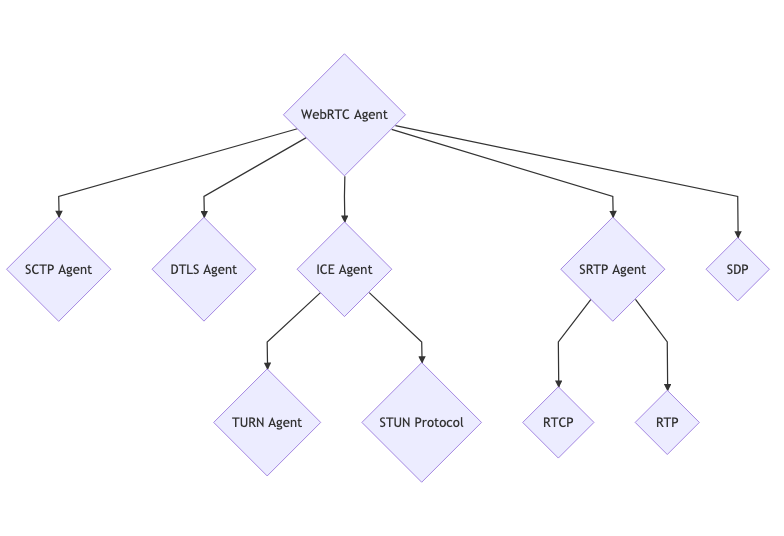
\includegraphics[width=0.75\textwidth]{webrtc-protocol-stack}}
  \caption{Protocoles employés par la technologie WebRTC}
  \label{fig:webrtc_protocols}
\end{figure}

La signalisation désigne le processus initial de mise en relation des pairs. 
Sans ce processus, une machine quelconque n’a aucune idée de qui voudrait bien la contacter. 
Pour ce faire, le protocole SDP est utilisé et permet la transmission d’informations capitales comme:

\begin{itemize}
  \item l’adresse \acrshort{ip} et le port de chaque agent \acrshort{webrtc} (plusieurs variantes, en réalité)
  \item les codecs multimédia supportés
  \item d’autres valeurs comme des certificats de sécurité nécessaires à la mise en place de la connexion et la sécurisation.
\end{itemize}


A la connexion, les agents \acrshort{webrtc} établissent un lien direct entre eux, sans intermédiaire. 
Face à la multitude de possibilités de connexion (couples constitués de l’adresse \acrshort{ip} et du port), 
le protocole \acrshort{ice} permet de choisir le meilleur candidat, en faisant recours au serveur \acrshort{stun} et parfois, à un serveur \acrshort{turn}. 
Le serveur \acrshort{turn} permet la retransmission des données lorsqu’il est impossible pour un agent \acrshort{webrtc} d'établir un lien 
direct avec un autre agent en raison de la configuration réseau (\acrshort{nat} et les types de liaisons possibles \cite{nat_links}).

Pour assurer la sécurité de la connexion, les protocoles \acrshort{dtls} et \acrshort{srtp} offrent une couche de chiffrement 
pour les contenus multimédia et les paquets brutes.

Enfin, les agents peuvent s'échanger de la donnée, du contenu multimédia, presque sans latence, grâce au protocoles \acrshort{rtp} et \acrshort{sctp}.

\acrshort{webrtc} est une technologie complexe qui requiert une certaine expertise quant à la connaissance des protocoles, 
leur utilisation et la mise en œuvre d'applications en temps réel. 
Elle sert de base aujourd’hui,  la plupart des applications de communication en temps réel.

\section{Software as a Service}
Parmi les modèles de distribution de logiciels, le SaaS représente une méthode ou le concepteur ou l'entité tenant l’application, 
l'héberge en ligne et la rend accessible à ses utilisateurs. 
En terme de commercialisation, il est possible d’offrir un accès à la plateforme moyennant un abonnement ou 
l’achat d’une version privée pour les besoins des corporations.

\section{Présentation de solutions existantes}
Plusieurs solutions s’inscrivent déjà dans le cadre du déroulement de cours en ligne en temps réel. 
Nous avons choisi quelques unes à passer en revue.

Il est important de préciser que les insuffisances relevées par rapport à ces outils ne sont aucunement d’ordre technique. 
Nous nous intéressons plutôt aux aspects logistique et financier. 
En effet, un des objectifs visés est de minimiser l’investissement requis pour la mise en place d’une solution de classe en ligne, 
tout en éliminant les barrières possibles.

\subsection{Google Classroom}
Google Classroom est un outil de la suite Google pour l'éducation. 
A défaut de disposer d’un module de visioconférence, il s'intègre parfaitement avec Google Meet (figure \ref{fig:g_meet}), à cette fin. 
L’application offre une version gratuite et dispose d’une interface accessible (figure \ref{fig:g_classrooms}). 
Toutefois, pour les réunions en ligne, le nombre maximum de connexions possibles se limite à 500 participants. 
Pour les entités universitaires dont l’effectif est considérable par classe, ceci pourrait présenter un désavantage. 
Grâce à la version payante néanmoins, on peut mettre en place un live stream, pour permettre d'accéder au contenu de 
la réunion sans toutefois pouvoir interagir avec les participants. 
Mais le modèle de souscription (figure \ref{fig:g_pricing}), basé sur le nombre d’utilisateurs risque d'entraîner des frais assez élevés.

% illustrations
\begin{figure}[h]
  \centering
  \frame{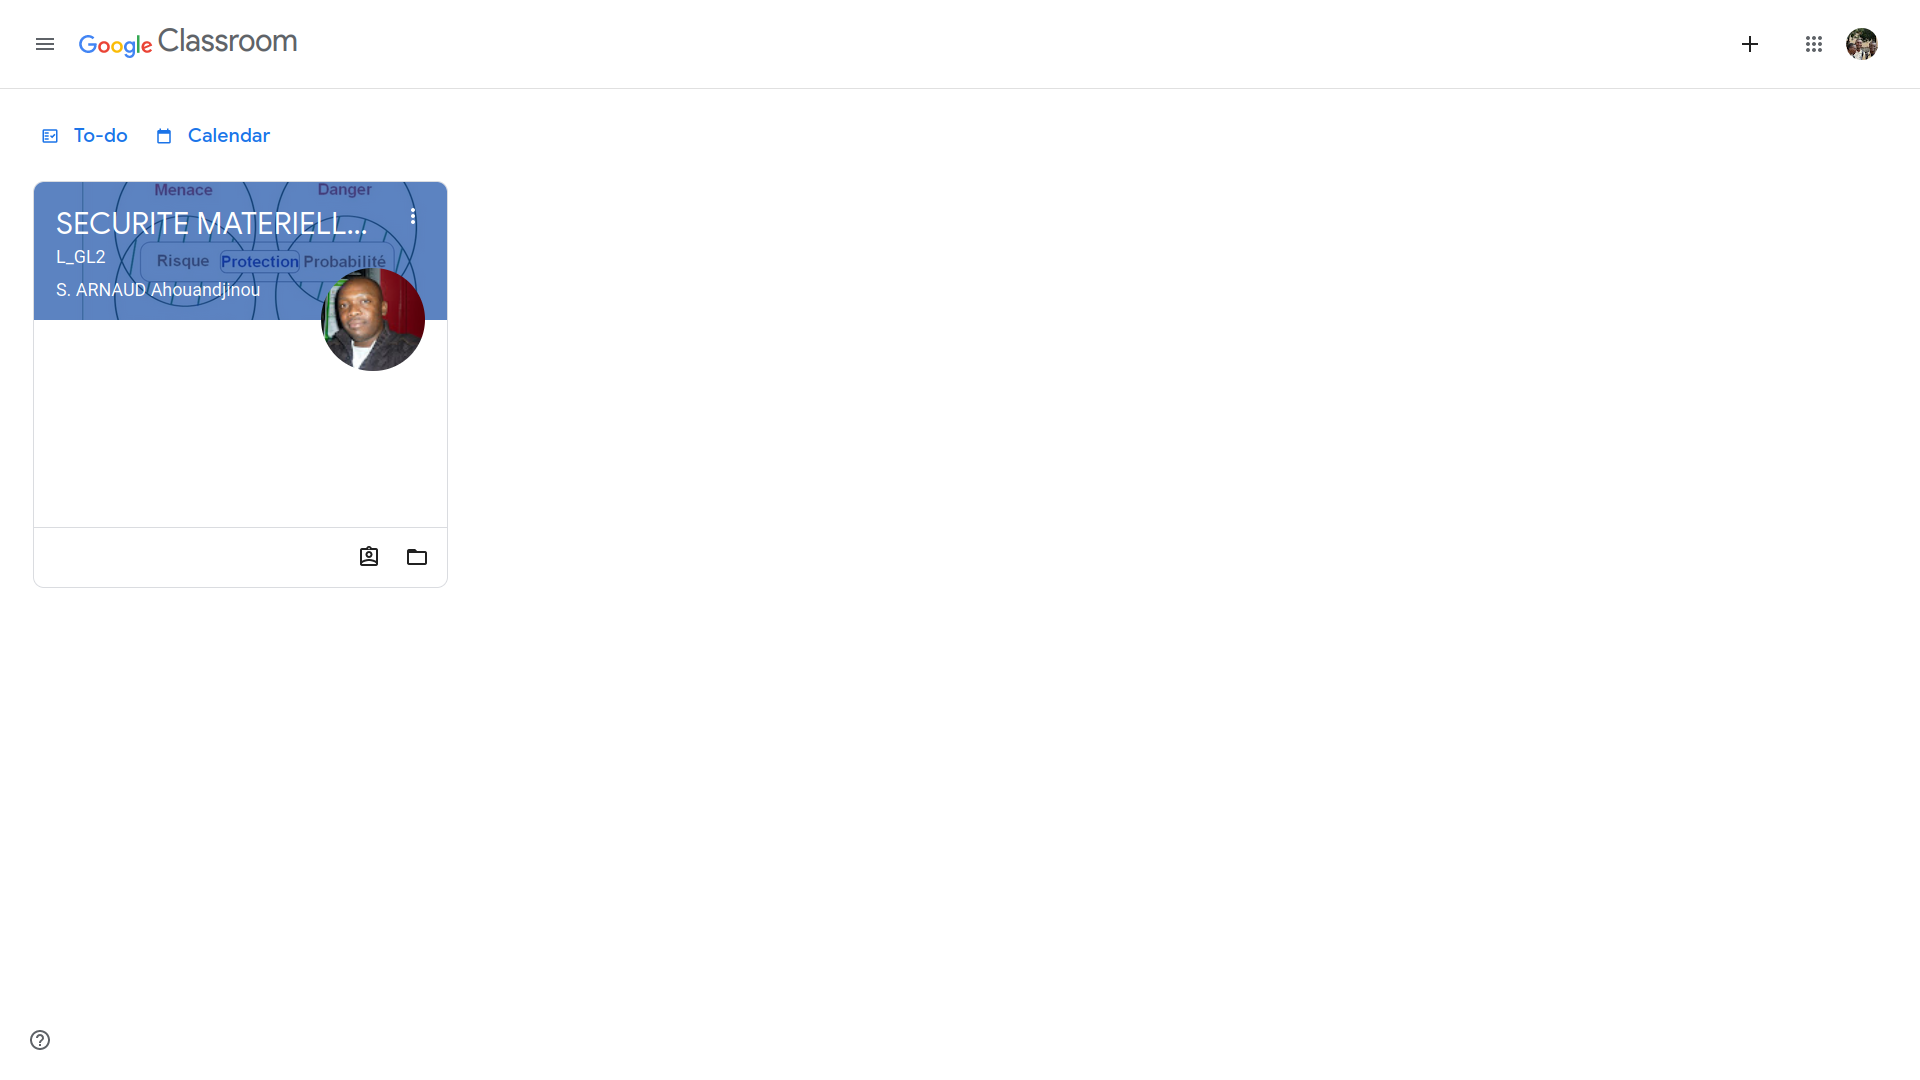
\includegraphics[width=0.75\textwidth]{g-classrooms}}
  \caption{Page d'acceuil de Google Classrooms avec un cas réel de cours}
  \label{fig:g_classrooms}
\end{figure}

\break

\begin{figure}[h]
  \centering
  \frame{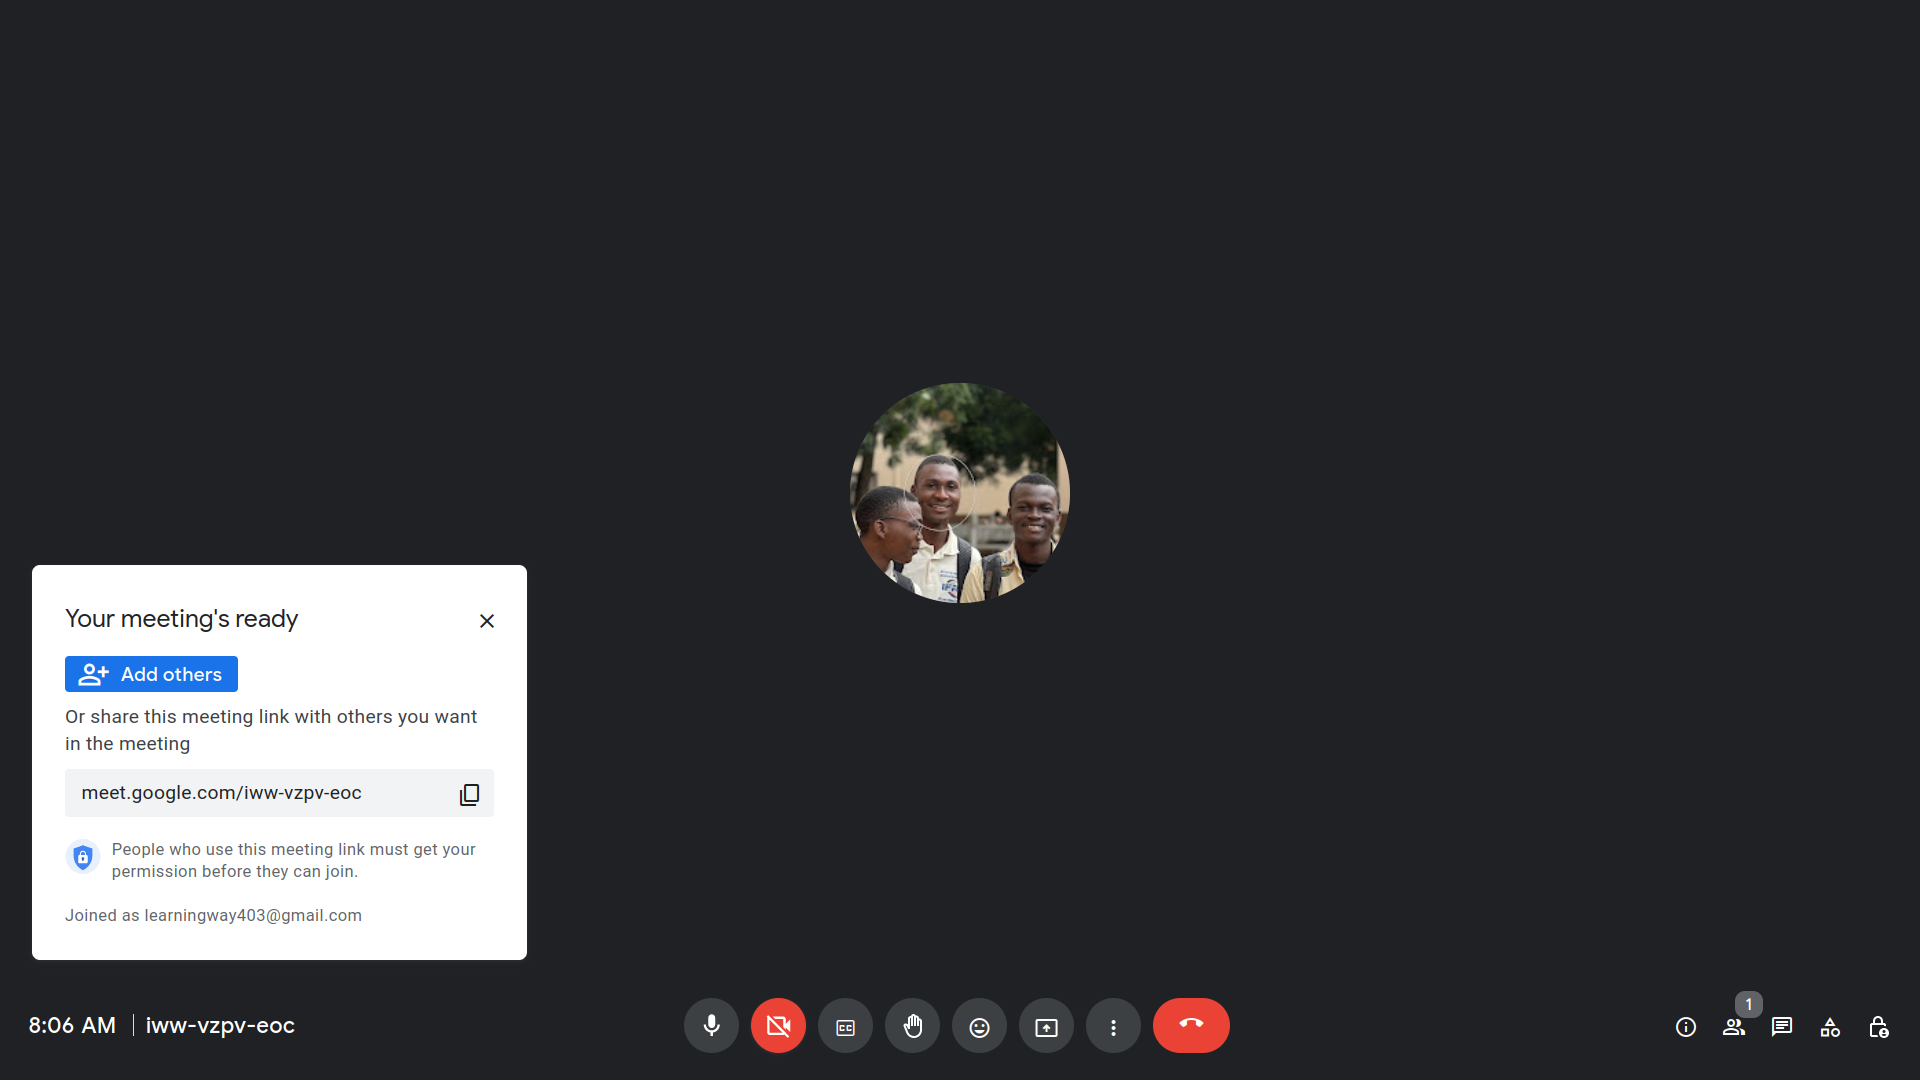
\includegraphics[width=0.75\textwidth]{g-meet}}
  \caption{Utilisation de Google Meet}
  \label{fig:g_meet}
\end{figure}
\begin{figure}[h]
  \centering
  \frame{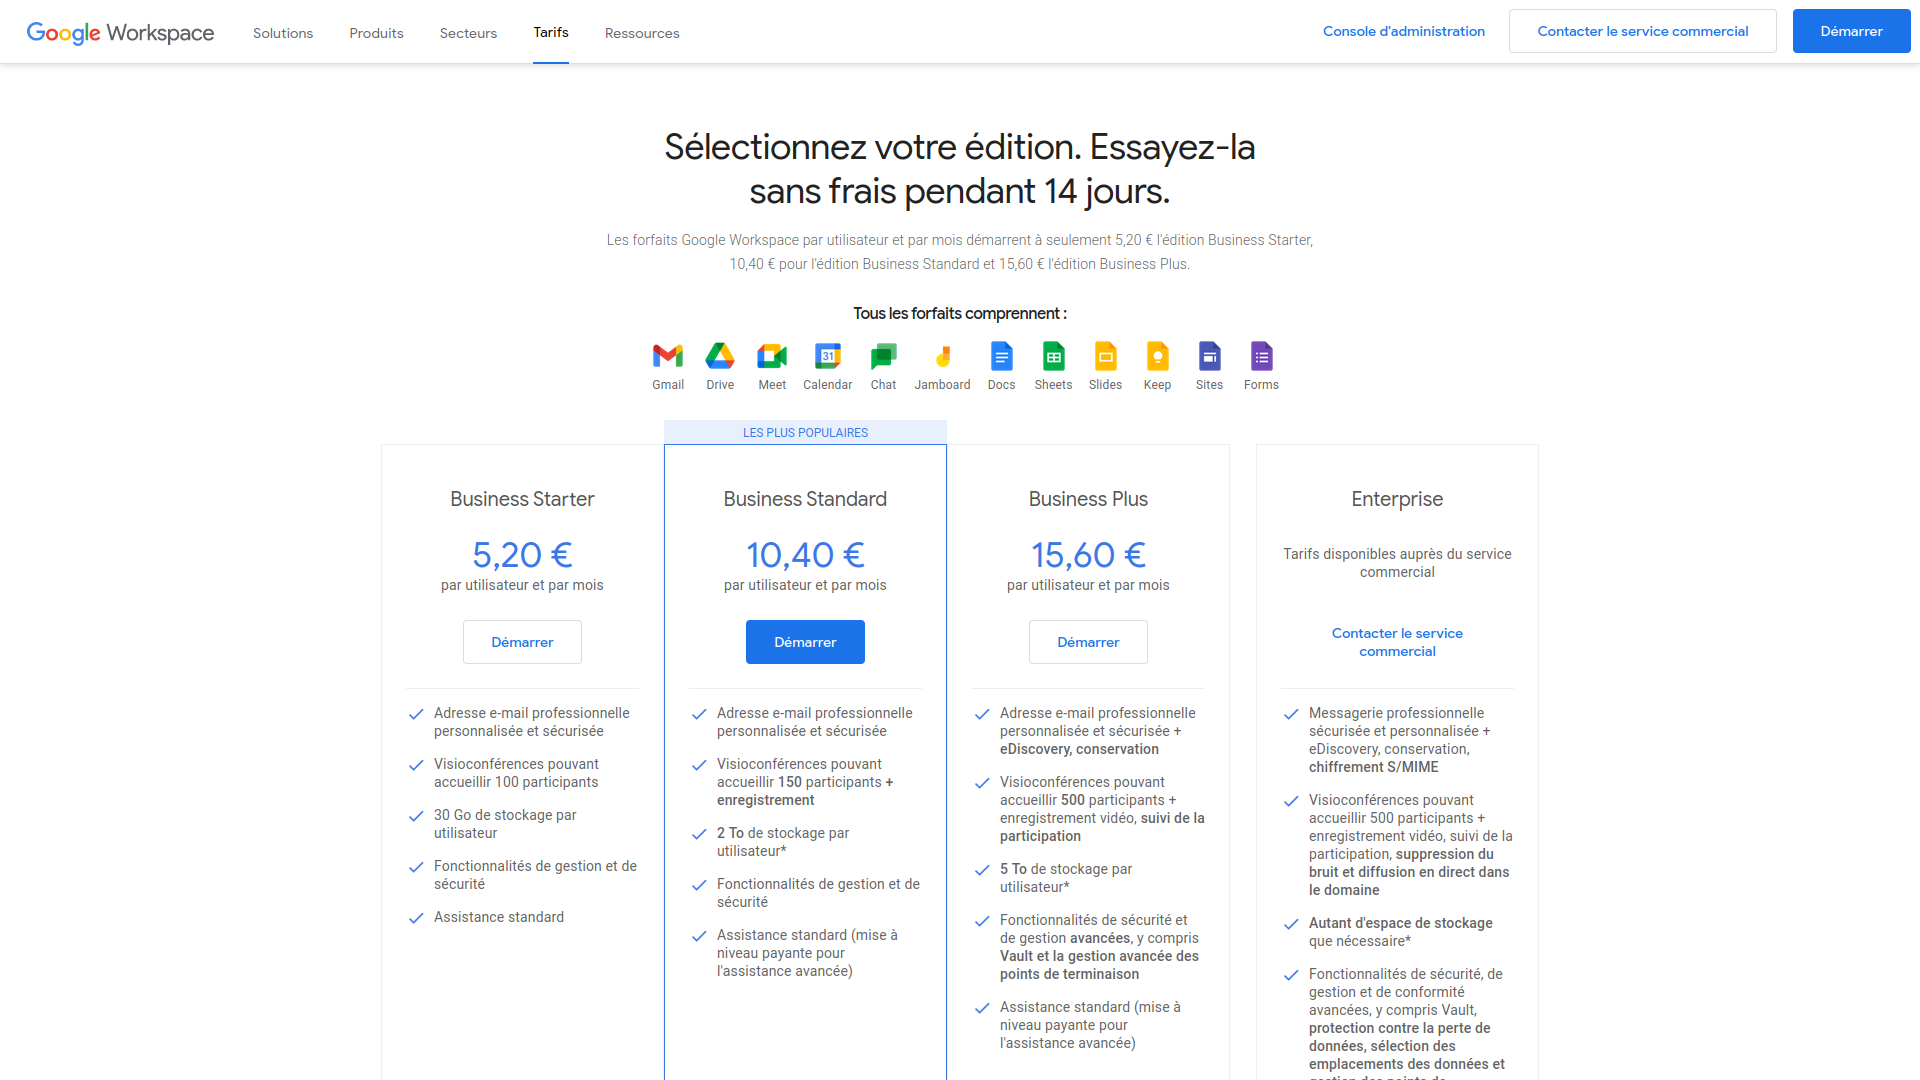
\includegraphics[width=0.75\textwidth]{gsuite-pricing-2023-02-17}}
  \caption{Offres de souscription à la suite Google pour éducation}
  \label{fig:g_pricing}
\end{figure}

\subsection{Zoom}
Zoom est un outil de communication très performant, qui a la capacité de supporter un grand nombre d’utilisateurs. 
Il dispose de fonctionnalités très utiles pour le déroulement de cours en ligne comme le partage d'écran ou le tableau virtuel. 
Accéder à ces fonctionnalités dans le cadre d’une utilisation à grande échelle requiert une souscription et les offres de Zoom ne sont pas des plus simples. 
En effet, Zoom dispose d’un panel large de services associés (figure \ref{fig:zoom_pricing}) et donc, sans orientation, 
il est possible de choisir une solution inadéquate en rapport avec le besoin, sans compter la perte financière.

% illustrations
\newpage
\begin{figure}[h]
  \centering
  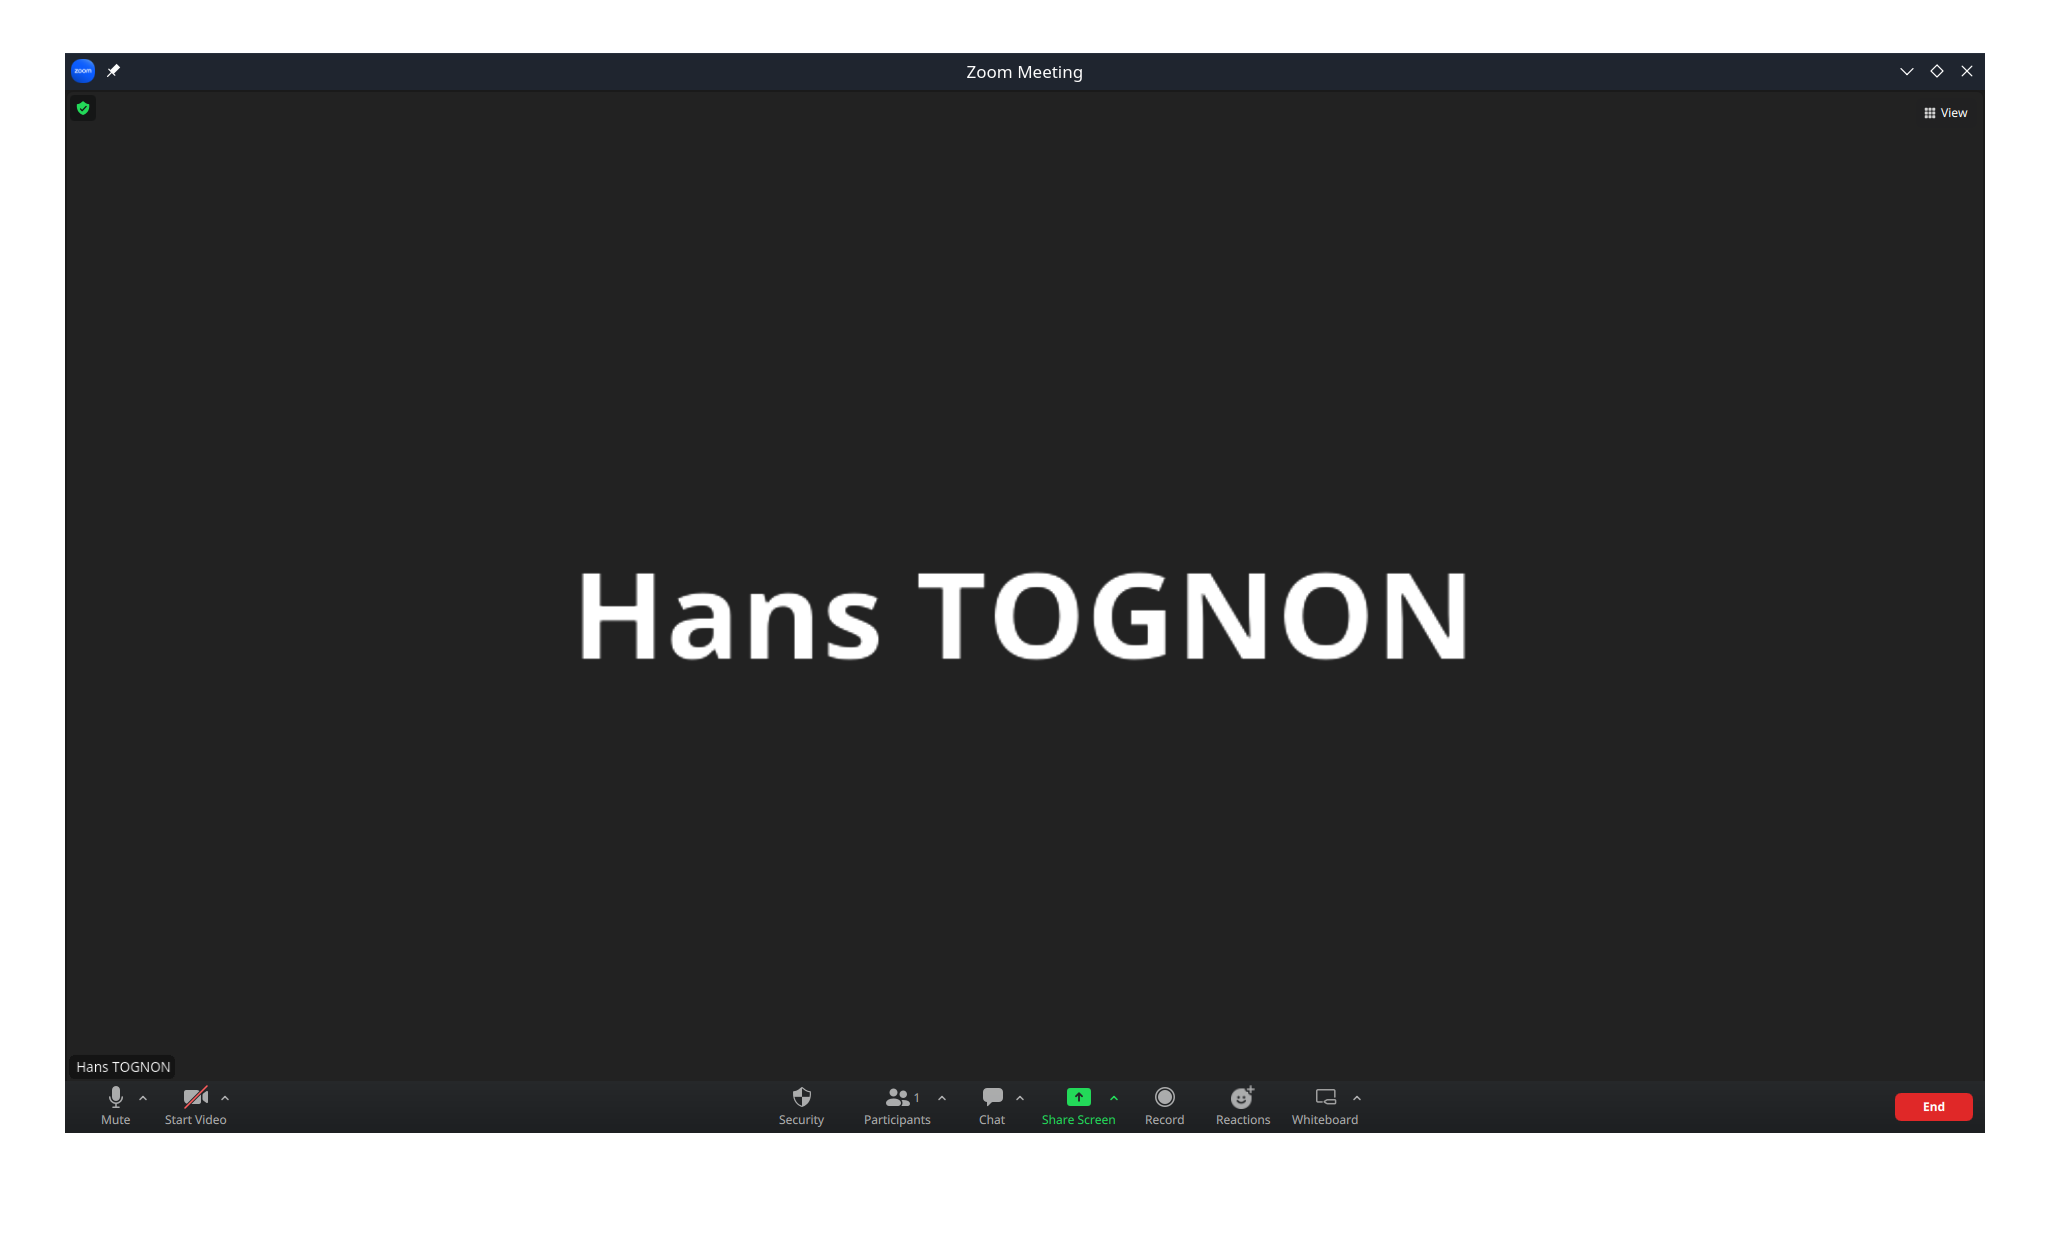
\includegraphics[width=0.75\textwidth]{zoom-meeting-ui}
  \caption{Interface de l'application Zoom}
  \label{fig:zoom_meeting_ui}
\end{figure}

\begin{figure}[h]
  \centering
  \frame{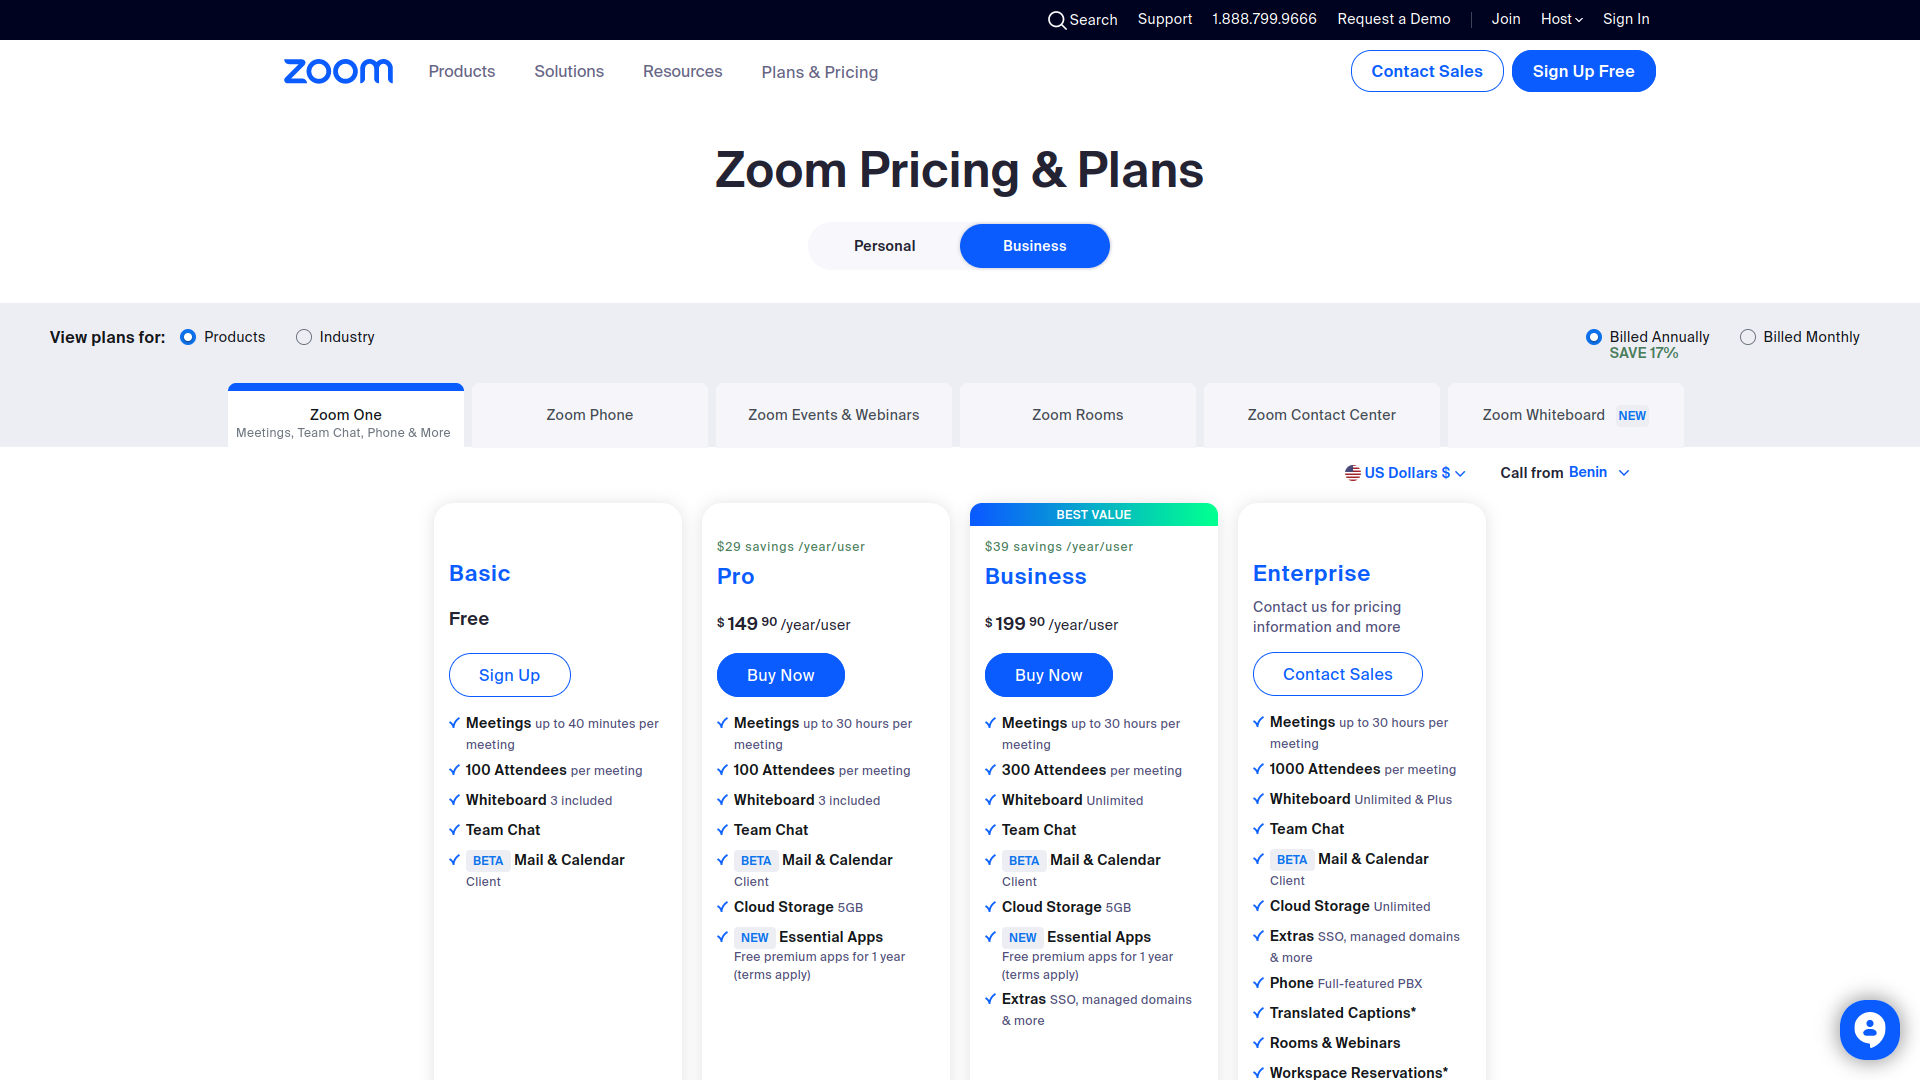
\includegraphics[width=0.75\textwidth]{zoom-pricing-2023-02-17}}
  \caption{Interface de l'application Zoom}
  \label{fig:zoom_pricing}
\end{figure}

\subsection{Moodle}
Moodle est un LMS Open Source populaire très connu et utilisé dans les entités de l’enseignement supérieur. 
Il peut être hébergé ou utilisé en ligne. 
Il offre un large panel de fonctionnalités et permet l'intégration de divers modules dont des modules de visio-conférence. 
BigBlueButton (figure \ref{fig:bbg_demo}) est une solution Open source employée à cet effet. 
La mise en place requiert toutefois, une certaine expertise et du matériel spécifique, ce qui en limiterait la portabilité.


% illustrations
\newpage
\begin{figure}[h]
  \centering
  \frame{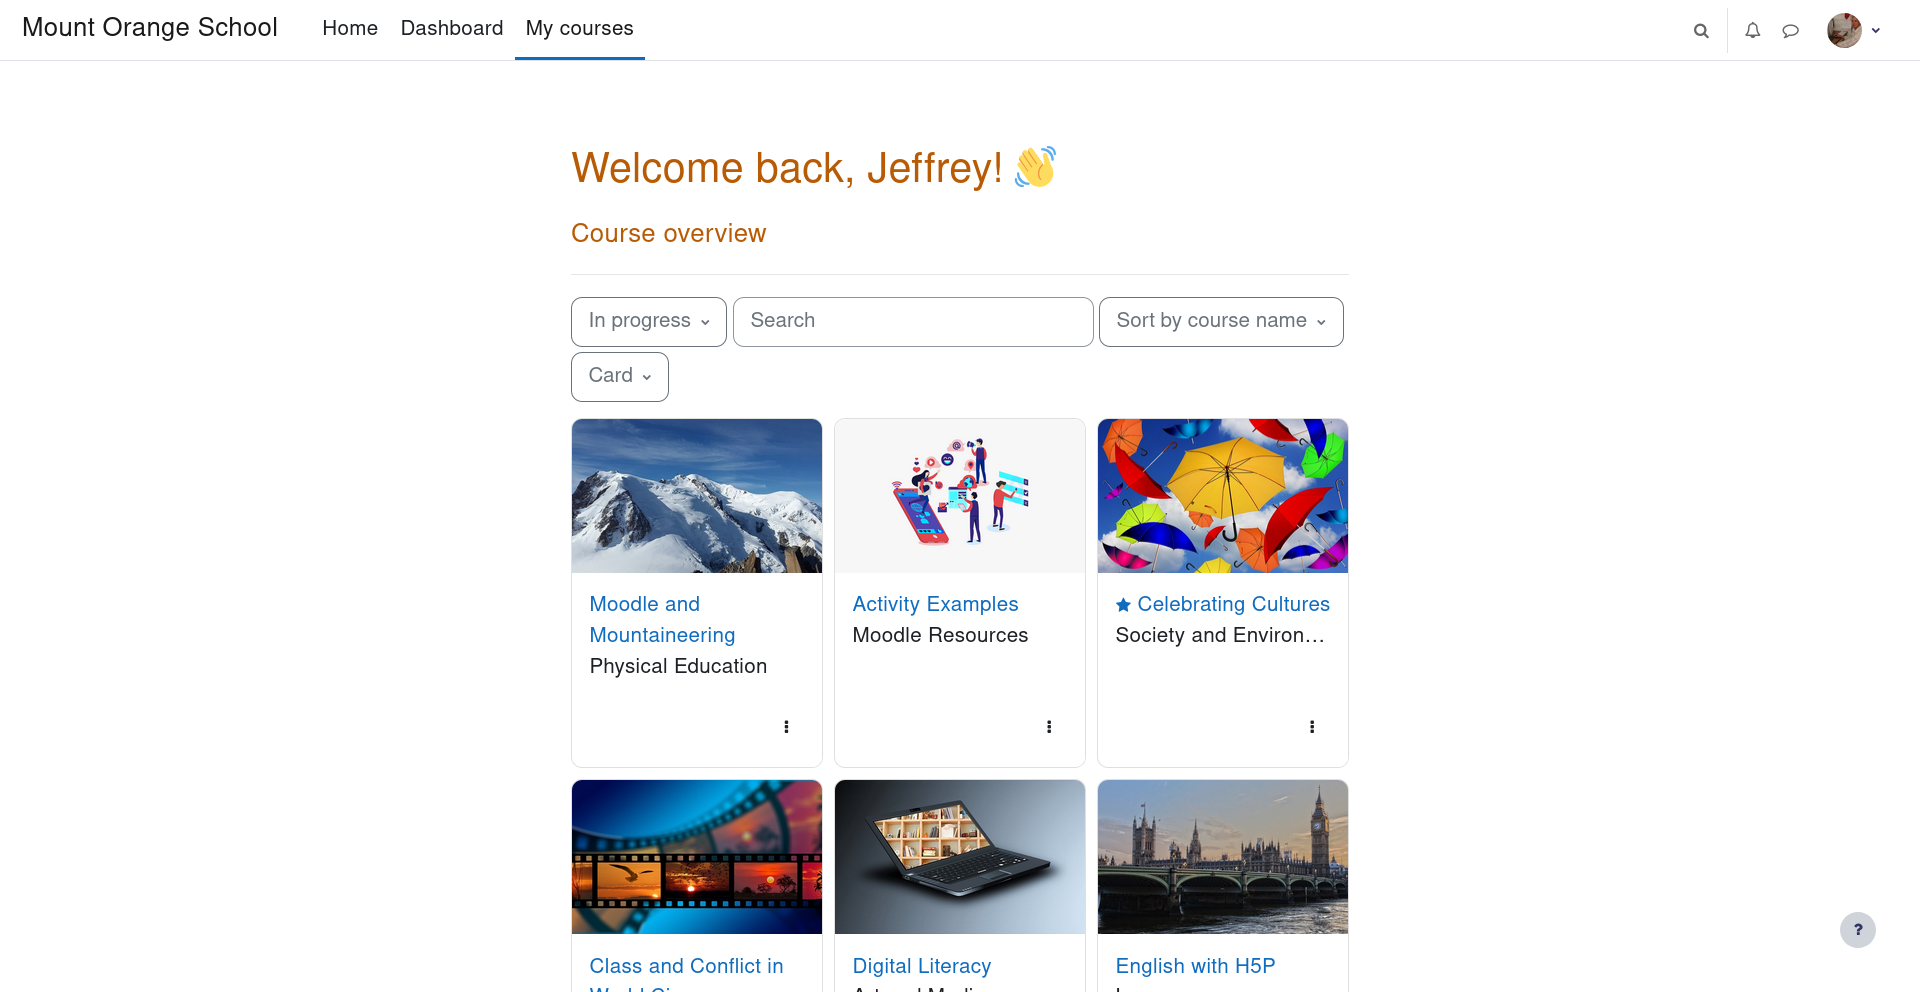
\includegraphics[width=0.75\textwidth]{moodle-demo-site}}
  \caption{Démonstration des capacités de Moodle}
  \label{fig:moodle_demo}
\end{figure}

\begin{figure}[h]
  \centering
  \frame{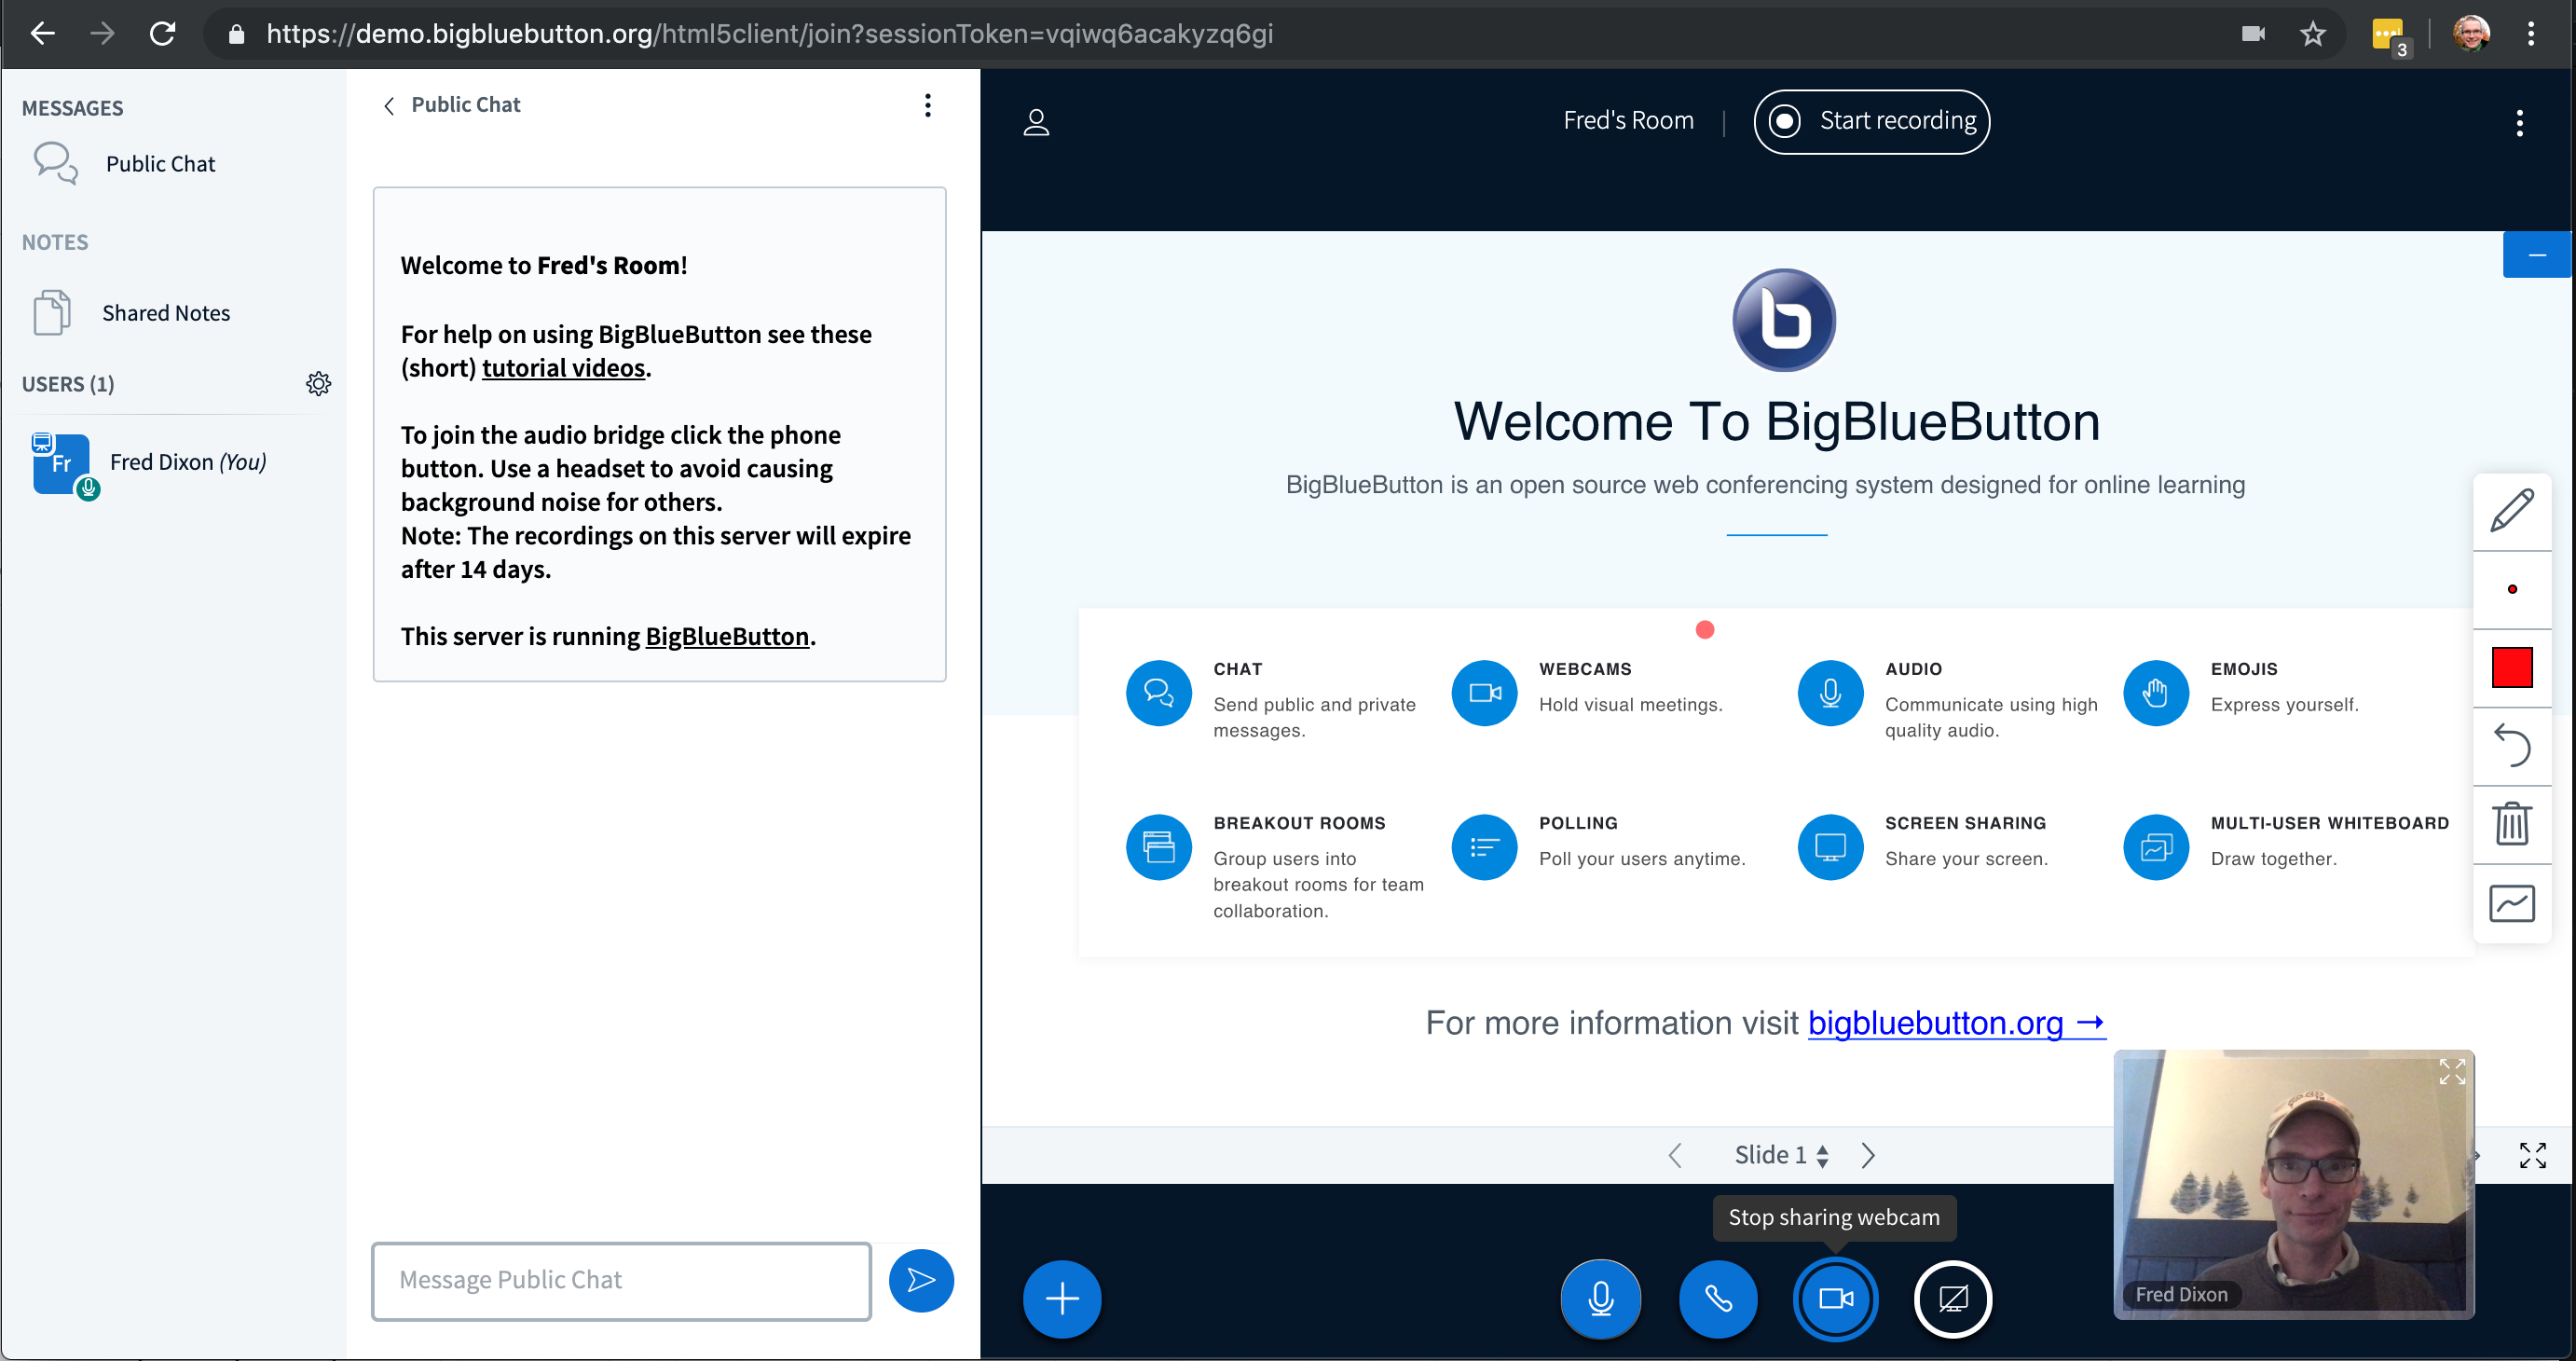
\includegraphics[width=0.75\textwidth]{big-blue-demo}}
  \caption{Démonstration de BigBlueButton}
  \label{fig:bbg_demo}
\end{figure}

\addcontentsline{toc}{section}{Conclusion}
\section*{Conclusion}
Ce chapitre a permis de faire une revue de l’existant et jette les bases des 
suivants en exposant les concepts clés qui seront développés. 
Les solutions suscitées conviendraient pour un usage modéré. 
Elles peuvent s'avérer coûteuses, pour peu qu’elles répondent au besoin. 
La solution que nous proposons vise à doter les organismes de l’enseignement supérieur, 
d’un moyen simple mais efficace de tenir les cours en ligne, offrant des outils d’assistance, 
tout en minimisant les coûts, que cela pourrait engendrer.
